\documentclass[journal,12pt,twocolumn]{IEEEtran}
%
\usepackage{setspace}
\usepackage{gensymb}
%\doublespacing
\singlespacing

%\usepackage{graphicx}
%\usepackage{amssymb}
%\usepackage{relsize}
\usepackage[cmex10]{amsmath}
%\usepackage{amsthm}
%\interdisplaylinepenalty=2500
%\savesymbol{iint}
%\usepackage{txfonts}
%\restoresymbol{TXF}{iint}
%\usepackage{wasysym}
\usepackage{amsthm}
%\usepackage{iithtlc}
\usepackage{mathrsfs}
\usepackage{txfonts}
\usepackage{stfloats}
\usepackage{bm}
\usepackage{cite}
\usepackage{cases}
\usepackage{subfig}
%\usepackage{xtab}
\usepackage{longtable}
\usepackage{multirow}
%\usepackage{algorithm}
%\usepackage{algpseudocode}
\usepackage{enumitem}
\usepackage{mathtools}
\usepackage{steinmetz}
\usepackage{tikz}
\usepackage{circuitikz}
\usepackage{verbatim}
\usepackage{tfrupee}
\usepackage[breaklinks=true]{hyperref}
%\usepackage{stmaryrd}
\usepackage{tkz-euclide} % loads  TikZ and tkz-base
%\usetkzobj{all}
\usetikzlibrary{calc,math}
\usepackage{listings}
    \usepackage{color}                                            %%
    \usepackage{array}                                            %%
    \usepackage{longtable}                                        %%
    \usepackage{calc}                                             %%
    \usepackage{multirow}                                         %%
    \usepackage{hhline}                                           %%
    \usepackage{ifthen}                                           %%
  %optionally (for landscape tables embedded in another document): %%
    \usepackage{lscape}     
\usepackage{multicol}
\usepackage{chngcntr}
%\usepackage{enumerate}

%\usepackage{wasysym}
%\newcounter{MYtempeqncnt}
\DeclareMathOperator*{\Res}{Res}
%\renewcommand{\baselinestretch}{2}
\renewcommand\thesection{\arabic{section}}
\renewcommand\thesubsection{\thesection.\arabic{subsection}}
\renewcommand\thesubsubsection{\thesubsection.\arabic{subsubsection}}

\renewcommand\thesectiondis{\arabic{section}}
\renewcommand\thesubsectiondis{\thesectiondis.\arabic{subsection}}
\renewcommand\thesubsubsectiondis{\thesubsectiondis.\arabic{subsubsection}}

% correct bad hyphenation here
\hyphenation{op-tical net-works semi-conduc-tor}
\def\inputGnumericTable{}                                 %%

\lstset{
%language=C,
frame=single, 
breaklines=true,
columns=fullflexible
}
%\lstset{
%language=tex,
%frame=single, 
%breaklines=true
%}

\begin{document}
%


\newtheorem{theorem}{Theorem}[section]
\newtheorem{problem}{Problem}
\newtheorem{proposition}{Proposition}[section]
\newtheorem{lemma}{Lemma}[section]
\newtheorem{corollary}[theorem]{Corollary}
\newtheorem{example}{Example}[section]
\newtheorem{definition}[problem]{Definition}
%\newtheorem{thm}{Theorem}[section] 
%\newtheorem{defn}[thm]{Definition}
%\newtheorem{algorithm}{Algorithm}[section]
%\newtheorem{cor}{Corollary}
\newcommand{\BEQA}{\begin{eqnarray}}
\newcommand{\EEQA}{\end{eqnarray}}
\newcommand{\define}{\stackrel{\triangle}{=}}

\bibliographystyle{IEEEtran}
%\bibliographystyle{ieeetr}


\providecommand{\mbf}{\mathbf}
\providecommand{\pr}[1]{\ensuremath{\Pr\left(#1\right)}}
\providecommand{\qfunc}[1]{\ensuremath{Q\left(#1\right)}}
\providecommand{\sbrak}[1]{\ensuremath{{}\left[#1\right]}}
\providecommand{\lsbrak}[1]{\ensuremath{{}\left[#1\right.}}
\providecommand{\rsbrak}[1]{\ensuremath{{}\left.#1\right]}}
\providecommand{\brak}[1]{\ensuremath{\left(#1\right)}}
\providecommand{\lbrak}[1]{\ensuremath{\left(#1\right.}}
\providecommand{\rbrak}[1]{\ensuremath{\left.#1\right)}}
\providecommand{\cbrak}[1]{\ensuremath{\left\{#1\right\}}}
\providecommand{\lcbrak}[1]{\ensuremath{\left\{#1\right.}}
\providecommand{\rcbrak}[1]{\ensuremath{\left.#1\right\}}}
\theoremstyle{remark}
\newtheorem{rem}{Remark}
\newcommand{\sgn}{\mathop{\mathrm{sgn}}}
\providecommand{\abs}[1]{\left\vert#1\right\vert}
\providecommand{\res}[1]{\Res\displaylimits_{#1}} 
\providecommand{\norm}[1]{\left\lVert#1\right\rVert}
%\providecommand{\norm}[1]{\lVert#1\rVert}
\providecommand{\mtx}[1]{\mathbf{#1}}
\providecommand{\mean}[1]{E\left[ #1 \right]}
\providecommand{\fourier}{\overset{\mathcal{F}}{ \rightleftharpoons}}
%\providecommand{\hilbert}{\overset{\mathcal{H}}{ \rightleftharpoons}}
\providecommand{\system}{\overset{\mathcal{H}}{ \longleftrightarrow}}
	%\newcommand{\solution}[2]{\textbf{Solution:}{#1}}
\newcommand{\solution}{\noindent \textbf{Solution: }}
\newcommand{\cosec}{\,\text{cosec}\,}
\providecommand{\dec}[2]{\ensuremath{\overset{#1}{\underset{#2}{\gtrless}}}}
\newcommand{\myvec}[1]{\ensuremath{\begin{pmatrix}#1\end{pmatrix}}}
\newcommand{\mydet}[1]{\ensuremath{\begin{vmatrix}#1\end{vmatrix}}}
%\numberwithin{equation}{section}
\numberwithin{equation}{subsection}
%\numberwithin{problem}{section}
%\numberwithin{definition}{section}
\makeatletter
\@addtoreset{figure}{problem}
\makeatother

\let\StandardTheFigure\thefigure
\let\vec\mathbf
%\renewcommand{\thefigure}{\theproblem.\arabic{figure}}
\renewcommand{\thefigure}{\theproblem}
%\setlist[enumerate,1]{before=\renewcommand\theequation{\theenumi.\arabic{equation}}
%\counterwithin{equation}{enumi}


%\renewcommand{\theequation}{\arabic{subsection}.\arabic{equation}}

\def\putbox#1#2#3{\makebox[0in][l]{\makebox[#1][l]{}\raisebox{\baselineskip}[0in][0in]{\raisebox{#2}[0in][0in]{#3}}}}
     \def\rightbox#1{\makebox[0in][r]{#1}}
     \def\centbox#1{\makebox[0in]{#1}}
     \def\topbox#1{\raisebox{-\baselineskip}[0in][0in]{#1}}
     \def\midbox#1{\raisebox{-0.5\baselineskip}[0in][0in]{#1}}

\vspace{3cm}


\title{Assignment 7}
\author{Jayati Dutta}





% make the title area
\maketitle

\newpage

%\tableofcontents

\bigskip

\renewcommand{\thefigure}{\theenumi}
\renewcommand{\thetable}{\theenumi}
%\renewcommand{\theequation}{\theenumi}


\begin{abstract}
This is a simple document explaining how to determine the foot of the perpendicular of any point on x-axis to a plane using Singular Value Decomposition.
\end{abstract}

%Download all python codes 
%
%\begin{lstlisting}
%svn co https://github.com/JayatiD93/trunk/My_solution_design/codes
%\end{lstlisting}

Download all and latex-tikz codes from 
%
\begin{lstlisting}
svn co https://github.com/gadepall/school/trunk/ncert/geometry/figs
\end{lstlisting}
%


\section{Problem}
Find the foot of the perpendicular from X-axis to the plane $3y-4z+7 =0$ using SVD.

\section{Explanation}
Let the given point on X-axis is $\myvec{p\\0\\0}$. Let us consider orthogonal vectors $\vec{m_1}$ and $\vec{m_2}$ to the normal vector $\vec{n}$.
Let $\vec{m}$=$\myvec{a\\b\\c}$ then $\vec{m}^T \vec{n}$=0.
\begin{multline}
\vec{m}^T \vec{n} = 0\\
\implies \myvec{a&b&c} \myvec{0\\3\\-4} = 0\\
\implies 0 a + 3b -4c = 0
\end{multline}
Now, for a=0 and b=4, c=3 and for a=1, b=0, c=0. So,
\begin{align}
m_1 = \myvec{0\\4\\3}\\
m_2 = \myvec{1\\0\\0}
\end{align}
Now,
\begin{align}
M = \myvec{0 & 1\\4 & 0\\3 & 0}
\end{align}
Now, we will solve $Mx=b$
\begin{multline}
\vec{M}\vec{x}=\vec{b}\\
\implies \myvec{0 & 1\\4 & 0\\3 & 0}\vec{x}= \myvec{p\\0\\0}
\label{eqn:2}
\end{multline}
Now the equation \ref{eqn:2} will be solved by using SVD.
$\vec{M}$ can be expressed as: $\vec{M}$ = $\vec{U} \vec{S} \vec{V}^T$.
Now, 
\begin{align}
\vec{M}^T \vec{M} = \myvec{0& 4& 3\\1 & 0 & 0} \myvec{0 & 1\\4 & 0\\3 & 0}\\
\implies \vec{M}^T \vec{M} = \myvec{25 & 0\\0 & 1}
\end{align}
Now, to get the eigen values of $\vec{M}^T \vec{M}$,
\begin{align}
\mydet{\vec{M}^T \vec{M} - \lambda I} = 0\\
\implies \mydet{25-\lambda & 0\\0 & 1-\lambda} = 0\\
\implies \lambda_1 = 25\\
\lambda_2 = 1
\end{align}
Now,
\begin{align}
S= \myvec{\sqrt{\lambda_1} & 0\\0 & \sqrt{\lambda_2}\\0 & 0}\\
S= \myvec{5 & 0\\0 & 1\\0 & 0}
\end{align}
So, the pseudo inverse of the diagonal matrix is:
\begin{align}
S_+= \myvec{\frac{1}{5} & 0 & 0\\0 & 1 & 0}
\end{align}
Now, the eigen vector of $\vec{M}^T \vec{M}$ for $\lambda_1$ = 25,
\begin{align}
\myvec{25-25 & 0\\0 & 1-25} \myvec{v_1\\v_2} = \myvec{0\\0}\\
\text{or,} \myvec{0 & 0\\0 & -24} \myvec{v_1\\v_2} = \myvec{0\\0}\\
\implies v_1 = 1\\
v_2 = 0
\end{align}
Now, the eigen vector of $\vec{M}^T \vec{M}$ for $\lambda_2$ = 1,
\begin{align}
\myvec{25-1& 0\\0 & 1-1} \myvec{v_3\\v_4} = \myvec{0\\0}\\
\text{or,} \myvec{24 & 0\\0 & 0} \myvec{v_3\\v_4} = \myvec{0\\0}\\
\implies v_3 = 0\\
v_4 = 1
\end{align}
So,
\begin{align}
\vec{V} = \myvec{1 & 0\\0 & 1}
\end{align}
Now,
\begin{align}
\vec{M} \vec{M}^T= \myvec{0 & 1\\4 & 0\\3 & 0}\myvec{0& 4& 3\\1 & 0 & 0} \\
\implies \vec{M} \vec{M}^T = \myvec{1 & 0 & 0\\0 & 16 & 12\\0 & 12 & 9}
\end{align}
Now, to get the eigen values of $\vec{M}\vec{M}^T$,
\begin{align}
\mydet{\vec{M}\vec{M}^T  - \lambda I} = 0\\
\implies \mydet{1-\lambda & 0 & 0\\0 & 16-\lambda & 12\\0 & 12 & 9-\lambda} = 0\\
\implies (1-\lambda)(\lambda^2 - 25\lambda)=0\\
\implies \lambda_1 = 0\\
\lambda_2 = 1\\
\lambda_3 = 25
\end{align}
Now, the eigen vector of $\vec{M}\vec{M}^T $ for $\lambda_1$ = 0,
\begin{align}
\myvec{1 & 0 & 0\\0 & 16 &12\\0 & 12 & 9} \myvec{u_1\\u_2\\u_3} = \myvec{0\\0\\0}\\
\end{align}
To get the row-reduced echelon form,
\begin{align}
\myvec{1 & 0 & 0\\0 & 16 &12\\0 &12&9} \xleftrightarrow[R_2\leftarrow\frac{R_2}{4}]{R_3\leftarrow \frac{R_3}{3}} \myvec{1 & 0 & 0\\0 & 4 &3\\0 &4&3}\\
\xleftrightarrow[]{R_3\leftarrow R_3-R_2}\myvec{1 & 0 & 0\\0 & 4 &3\\0 &0&0}
\end{align}
So,
\begin{align}
\myvec{1 & 0 & 0\\0 & 4 &3\\0 &0&0}\myvec{u_1\\u_2\\u_3} = \myvec{0\\0\\0}\\
\implies \vec{u_1}=0\\
\vec{u_2}=-3\\
\vec{u_3}=4
\end{align}
Now, the eigen vector of $\vec{M}\vec{M}^T $ for $\lambda_2$ = 1,
\begin{align}
\myvec{0 & 0 & 0\\0 & 15 &12\\0 & 12 & 8} \myvec{u_4\\u_5\\u_6} = \myvec{0\\0\\0}\\
\end{align}
To get the row-reduced echelon form,
\begin{align}
\myvec{0 & 0 & 0\\0 & 15 &12\\0 & 12 & 8} \xleftrightarrow[R_2\leftarrow\frac{R_2}{3}]{R_3\leftarrow \frac{R_3}{4}} \myvec{0 & 5 & 4\\0 &3 &2\\0 &0&0}\\
\xleftrightarrow[]{R_2\leftarrow R_2-R_1}\myvec{0 & 5 & 4\\0 &-2 &-2\\0 &0&0}\\
\xleftrightarrow[]{R_2\leftarrow \frac{R_2}{-2}}\myvec{0 & 5 & 4\\0 &1 &1\\0 &0&0}\\
\xleftrightarrow[]{R_2\leftarrow 5 R_2 - R_1}\myvec{0 & 5 & 4\\0 &0 &1\\0 &0&0}
\end{align}
So,
\begin{align}
\myvec{0 & 5 & 4\\0 &0 &1\\0 &0&0}\myvec{u_4\\u_5\\u_6} = \myvec{0\\0\\0}\\
\implies \vec{u_4}=1\\
\vec{u_5}=0\\
\vec{u_6}=0
\end{align}
Similarly, the eigen vector of $\vec{M}\vec{M}^T $ for $\lambda_3$ = 25,
\begin{align}
\myvec{-24 & 0 & 0\\0 &3 &-4\\0 &0&0}\myvec{u_7\\u_8\\u_9} = \myvec{0\\0\\0}\\
\implies \vec{u_7}=0\\
\vec{u_8}=4\\
\vec{u_9}=3
\end{align}
Now,
\begin{align}
\vec{U} = \myvec{0 & 1 & 0\\-3 & 0 & 4\\4 & 0 & 3}\\
\implies \vec{U}^T = \myvec{0 & -3 & 4\\1 & 0 & 0\\0 & 4 & 3}\\
\end{align}
\begin{align}
\vec{X} = \vec{V} \vec{S_+} \vec{U}^T \vec{b}
\end{align}
Now,
\begin{align}
\vec{U}^T \vec{b} = \myvec{0\\p\\0}\\
\vec{S_+} \vec{U}^T \vec{b} = \myvec{0\\ p}\\
\vec{V} \vec{S_+} \vec{U}^T \vec{b} = \myvec{0 \\ p}\\
\vec{X}= \myvec{0\\p}
\label{eqn:3}
\end{align}
So, $\vec{X}$=$\myvec{0\\p}$.\\
Verifying the solution of \ref{eqn:3} using,
\begin{align}
\vec{M}^T \vec{M} \vec{X} = \vec{M}^T \vec{b}\\
\implies \myvec{25 & 0\\0 & 1}\vec{X} = \myvec{0\\p}
\end{align}
Now, taking the augmented matrix,
\begin{align}
\myvec{25 & 0 & 0\\0 & 1 & p} \xleftrightarrow[]{R_1\leftarrow \frac{R_1}{25}}\myvec{1 & 0 & 0\\0 & 1 & p}\\
\implies \myvec{1 & 0\\0 & 1}\vec{X}=\myvec{0\\p}
\end{align}
So we can conclude that the solution is verified.

Now, the plane $3y-4z+7 =0$ is parallel to x-axis. Another plane that is perpendicular to the above plane and passing through x-axis is $4y+3z=0$ which intersects the above plane at a straight $4y+3z=-\frac{7}{25}$ and the point $p$ will be on that line of the plane as the perpendicular distance of the plane $3y-4z+7 =0$ from x-axis is $\frac{7}{25}$.

\begin{figure}[!ht]
\centering
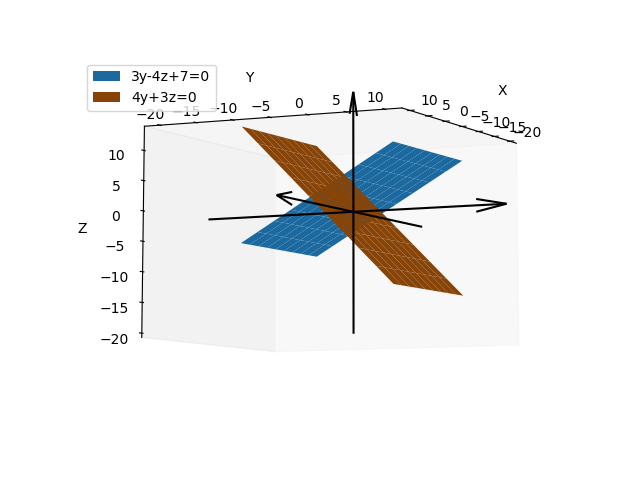
\includegraphics[width=\columnwidth]{./figs/perperndi_foot_1.png}
\caption{Perpendicular surfaces}
\label{fig:Perpendicular surfaces}
\end{figure} 

\begin{figure}[!ht]
\centering
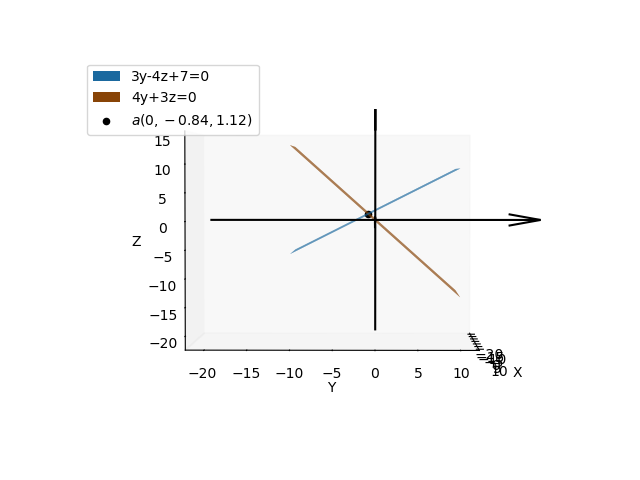
\includegraphics[width=\columnwidth]{./figs/perperndi_foot_2.png}
\caption{Perpendicular surfaces}
\label{fig:Perpendicular surfaces_point}
\end{figure}

Now,
\begin{align}
3y-4z+7 =0\\
4y+3z=0
\end{align}
From these 2 equations we get 
\begin{align}
\myvec{3&-4\\4&3} \myvec{y\\z} = \myvec{-7\\0}
\end{align}
Now, the augmented matrix is $\myvec{3&-4&-7\\4&3\\0}$
\begin{align}
\myvec{3&-4&-7\\4&3&0} \xleftrightarrow[R_1\leftarrow \frac{R_1}{3}]{R_2\leftarrow \frac{R_2}{4}}\myvec{1&-\frac{4}{3}&-\frac{7}{3}\\1&\frac{3}{4}&0}\\
\xleftrightarrow[]{R_2\leftarrow R_2-R_1}\myvec{1&-\frac{4}{3}&-\frac{7}{3}\\0&\frac{25}{12}&\frac{7}{3}}\\
\implies z= \frac{28}{25}\\
y= -\frac{21}{25}
\end{align}

In this case, the co-ordinate of the point on the plane $3y-4z+7 =0$ does not depend on any value of x. This fact is verified through the plot \ref{fig:Perpendicular surfaces_point}.
%\renewcommand{\theequation}{\theenumi}
%\begin{enumerate}[label=\thesection.\arabic*.,ref=\thesection.\theenumi]
%\numberwithin{equation}{enumi}
%\item Verification of the above problem using python code.\\
%\solution The  following Python code generates Fig. \ref{fig:hyperbola}
%\begin{lstlisting}
%codes/hyperbola_3.py
%\end{lstlisting}
%%
%\end{enumerate}

\end{document}



